\documentclass[a4paper, 12pt]{article}
\usepackage{graphicx}
\usepackage{verbatim}
% \usepackage{lstlisting}
\usepackage{subfig}
\usepackage{float}
 \usepackage[spanish]{babel}   %ver bien como es
\usepackage[utf8]{inputenc}

\begin{document}

\tableofcontents

\newpage


\begin{center}
\section*{Aclaraciones Generales}
\addcontentsline{toc}{section}{Aclaraciones Generales} 

\begin{itemize}
\item La implementaci\'on de todos los algoritmos se realiz\'o en lenguaje C++.

\item Para calcular los tiempos de ejecuci\'on de los algoritmos se utiliz\'o la funci\'on gettimeofday(), que se encuentra en la librer\'ia $<sys/time.h>$. Dado que dicha funci\'on funciona solamente en sistemas operativos de tipo linux, se debe compilar con el flag -DTIEMPOS en este tipo de sistemas para poder hacer uso de las mismas.

\item Para la realizaci\'on de los gr\'aficos se utiliz\'o Qtiplot
\end{itemize}

\end{center}

\newpage
\begin{center}
\section*{Ejercicio 1: Matching Máximo}
\addcontentsline{toc}{section}{Ejercicio 1: Matching Máximo} 
\end{center}
 
\subsection*{Introducción}
\addcontentsline{toc}{subsection}{Introducción} 
En este ejercicio se pedía encontrar el peso de un matching de peso máximo dentro de un grafo. Se define como matching a un subconjunto de aristas que no comparten vértices. Si bien este ejercicio podría ser de gran complejidad, el mismo se encuentra en una presentación m\'as accesible dado que no hay que aplicar el algoritmo sobre cualquier tipo de grafos, sino que solamente tiene que ser aplicable a grafos de 3 o más nodos que sean ciclos simples, es decir, grafos que en su isomorfismo planar sean simplemente un dibujo de un polígono.

% aca podria ir algun dibujo de como serian los grafos a ver y como seria algun grafo que no hay que analizar.

\subsection*{Algoritmo}
\addcontentsline{toc}{subsection}{Algoritmo} 



El algoritmo propuesto como resolución del problema consiste en transformar el grafo en un vector, dado que al poder ser representado como un polígono, se puede ver que, quitando una sola arista, el grafo se convierte en una sucesión de aristas con peso, lo cual se puede representar con un vector de números. La idea del algoritmo es poder encontrar el máximo matching posible, una primera aproximación a la solución final, podría ser la siguiente:

\begin{enumerate}
\item Se toma una arista cualquiera para comenzar. Luego, el matching buscado tiene dos opciones: contener esa arista, o no contenerla. Entonces el resultado será el máximo entre:
\begin{itemize}
 \item El matching máximo del grafo sin esa arista (no se utiliza la primer arista tomada).
 \item El matching máximo del grafo sin esa arista, ni ninguna de sus dos aristas vecinas, más el valor de la arista elegida en primer término (si se utiliza la primer arista tomada).
\end{itemize}
  De esta manera, el problema sobre un grafo, se convierte en 2 problemas similares pero sobre vectores.
\item En este momento, se necesita sacar el matching máximo, pero sobre vectores, para hacer esto se piensa de manera parecida al punto anterior comenzando con el último elemento: o bien el matching máximo lo contiene, o bien no lo contiene. Luego, el matching buscado para el vector, sera el máximo entre el matching máximo del vector sin el último elemento (caso en el que no se usa el último elemento) y el matching máximo del vector sin los últimos dos elementos más el valor del último elemento (caso en el que sí se utiliza el último).

	$matchingMaximo(v_1,v_2,..,v_n) = \\ maximo(matchingMaximo(v_1,v_2,..,v_{n-1}), \\ matchingMaximo(v_1,v_2,..,v_{n-2}) + v_n)$
\item De esta manera, se puede ver que el problema se torna recursivo, siendo solucionado mediante la técnica de dividir y conquistar, teniendo como caso base los vectores de dos o un elemento resolubles trivialmente.
\end{enumerate}

Si bien el algoritmo propuesto retorna el valor esperado, la complejidad del mismo no es óptima. Al hacer los llamados recursivos sucede que hay varios matching máximos que se realizan sobre los mismos vectores, generando así más cálculos de los necesarios. Fue por esto, que el siguiente paso fue modificar el algoritmo para que no calcule las cosas de modo \emph{top down}, sino que fuese un algoritmo \emph{bottom up}, para así evitar los cálculos repetidos, utilizando así la mayor ventaja de la programación dinámica, técnica que define al algoritmo final.

De esta manera, se pensó como teniendo instancias más peque~{n}as del problema, se puede conocer la solución de una instancia mayor. Se utilizó que, dadas las soluciones óptimas para vectores de n-2 y n-1 elementos, la solución para el vector de n elementos es el máximo entre la solución de n-1 elementos, y la solución de n-2 elementos más el elemento n-ésimo. Es así que el cálculo se torna \emph{bottom up}, calculando los máximos de los subvectores, una sola vez.

A continuación se muestra el pseudocódigo del algoritmo propuesto como resolución del problema.


% \begin{lstlisting}
\begin{verbatim}
matchingMaximo(grafo G)
   tomar v una arista cualquiera
   tomar u y w vecinos de v
   res := max(matchingSobreVector(G-u-v-w) + v, 
          matchingSobreVector(G-v))

matchingSobreVector(Vector peso_arista)
si tamanio(peso_arista) = 0
   devolver 0
si tamanio(peso_arista) = 1
   devolver peso_arista[1]
si tamanio(peso_arista) = 2
   devolver max(peso_arista[1], peso_arista[2])
si tamanio(peso_arista) >= 3
   peso_maximo_hasta_i-1 := max(peso_arista[1], peso_arista[2]) 
   peso_maximo_hasta_i-2 := peso_arista[1]
   Para i = 3 hasta n {
      temp := peso_maximo_hasta_i-1
      peso_maximo_hasta_i-1 := 
         max( peso_maximo_hasta_i-2 + peso_arista[i], peso_maximo_hasta_i-1)
      peso_maximo_hasta_i-2 := temp
   }
   devolver peso_maximo_hasta_i-1

\end{verbatim}
% \end{lstlisting}

A continuación se presenta un seguimiento del algoritmo sobre un ciclo simple de siete aristas.

\begin{figure}[H]
\begin{center}
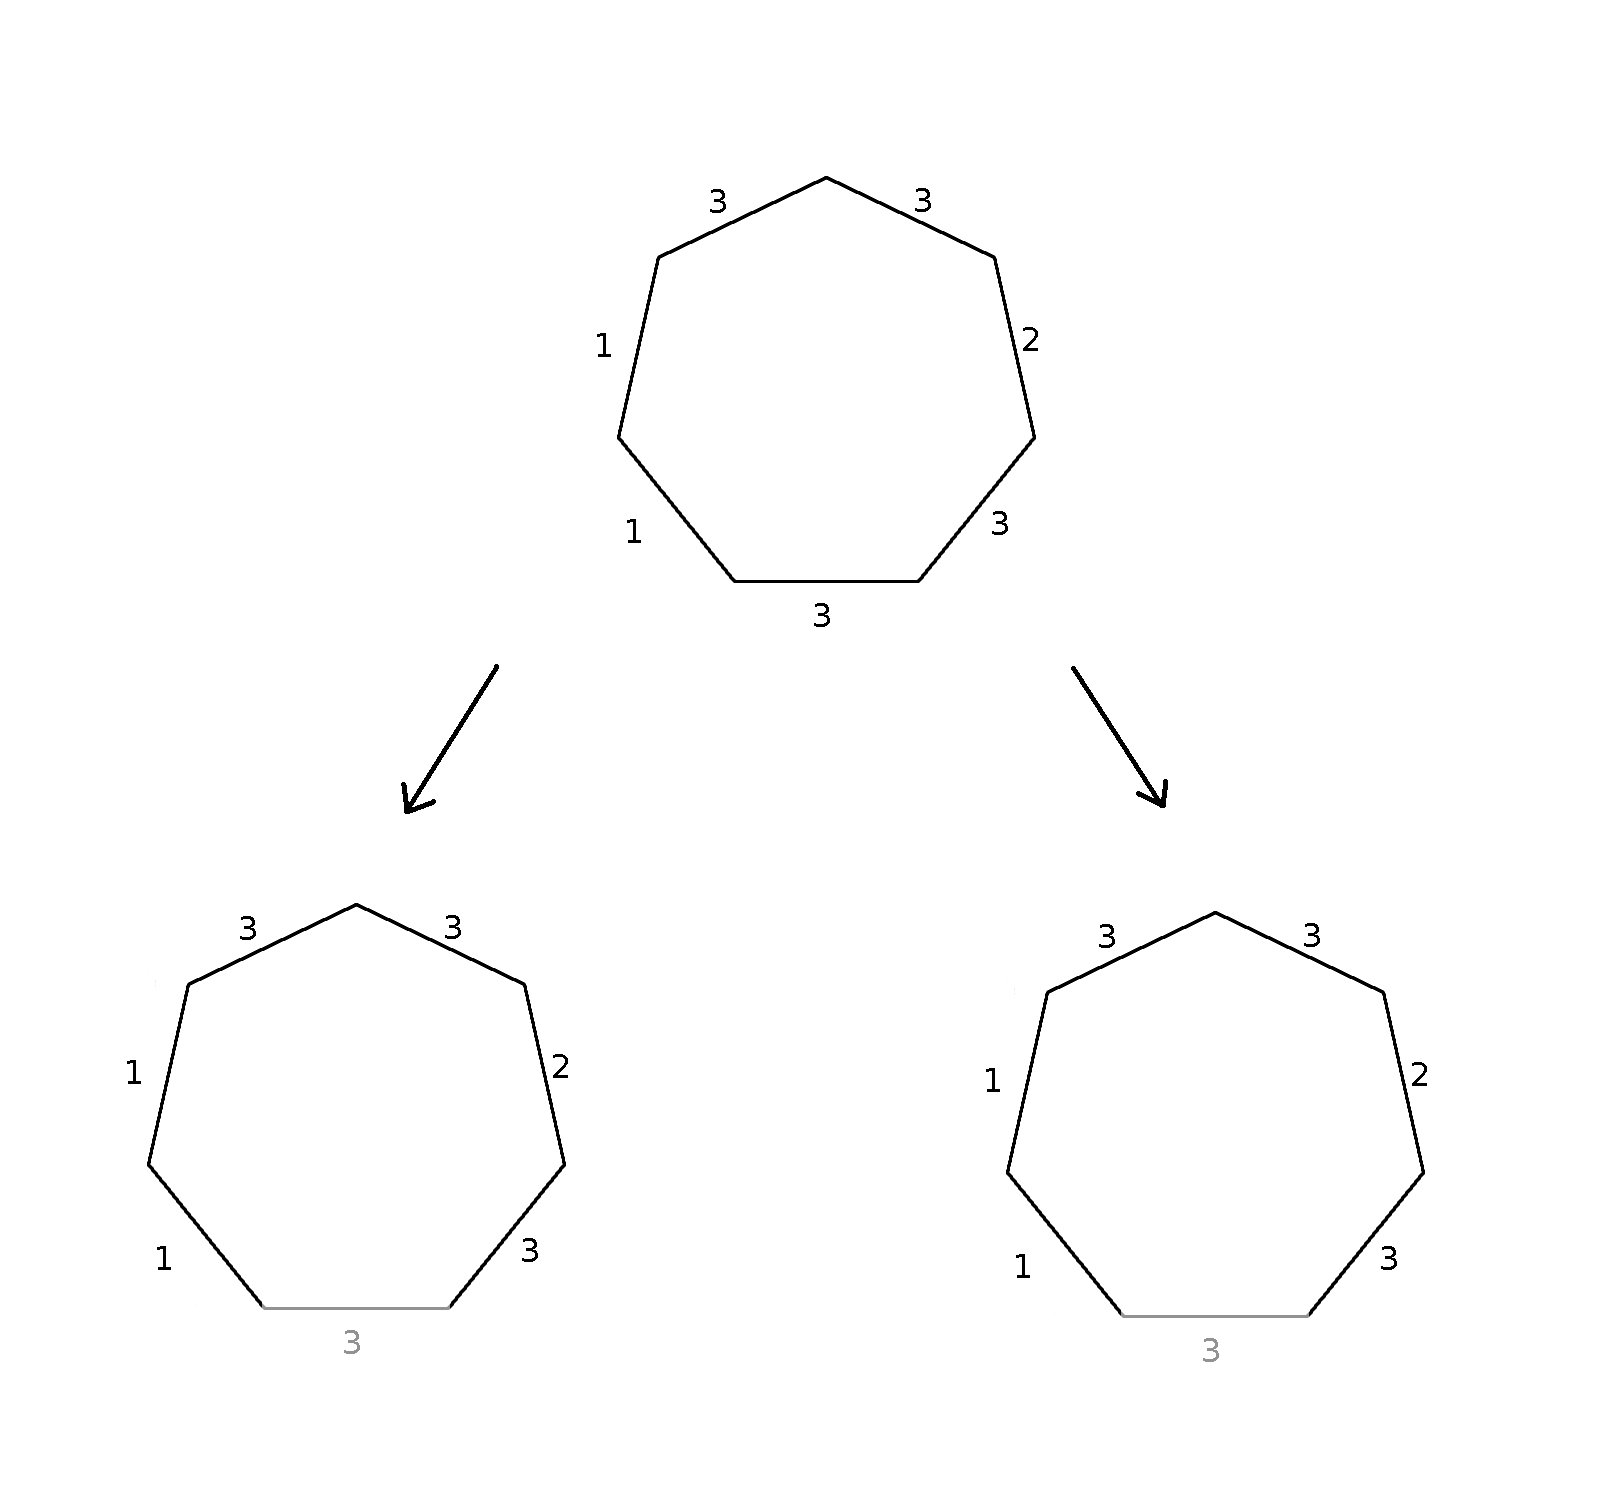
\includegraphics[width=0.7\textwidth]{imagenes/paso1y2.png}
\caption{Se toma la arista inferior y se bifurca entre utilizar la misma o no}
\end{center}
\end{figure}

\begin{figure}[H]
\centering
\subfloat{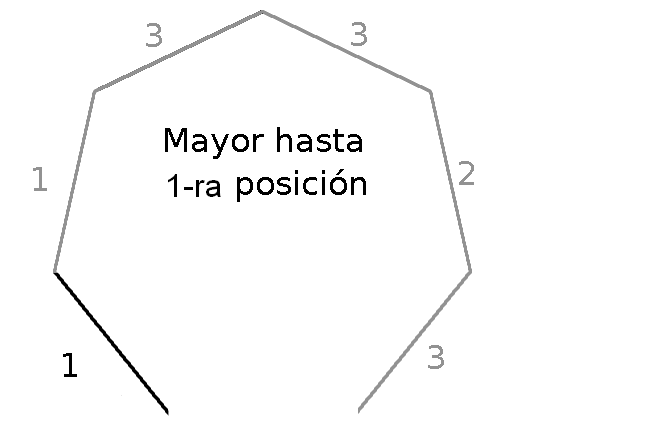
\includegraphics[width=0.3\textwidth]{imagenes/paso0b.PNG}}
\qquad
\subfloat{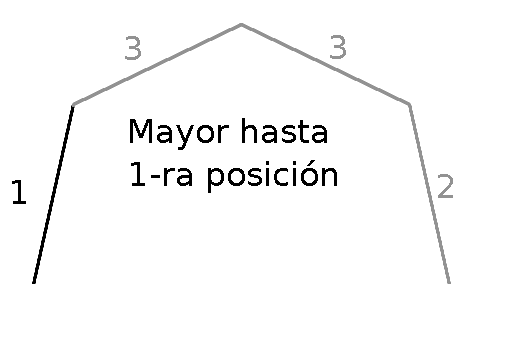
\includegraphics[width=0.3\textwidth]{imagenes/paso3a.png}}
\caption{Se calcula el matching máximo en los vectores - Primer paso}
\end{figure}

\begin{figure}[H]
\centering
\subfloat{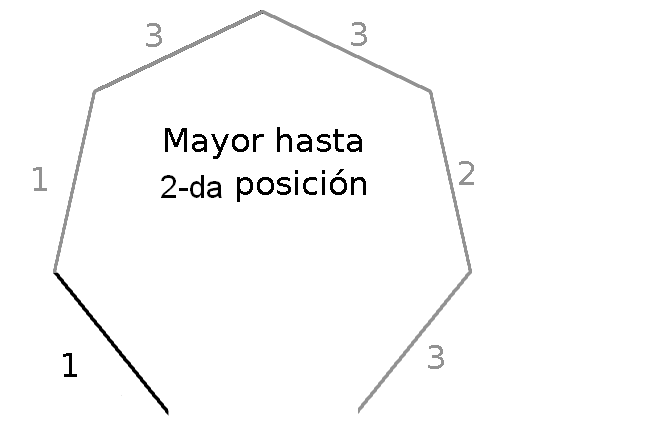
\includegraphics[width=0.3\textwidth]{imagenes/paso1b.PNG}}
\qquad
\subfloat{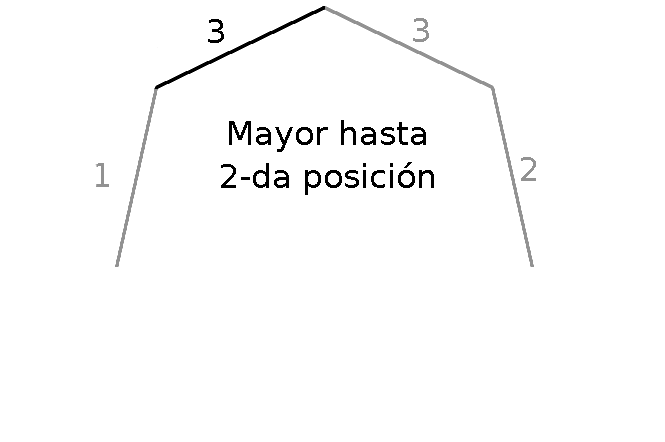
\includegraphics[width=0.3\textwidth]{imagenes/paso4a.png}}
\caption{Se calcula el matching máximo en los vectores - Segundo paso}
\end{figure}

\begin{figure}[H]
\centering
\subfloat{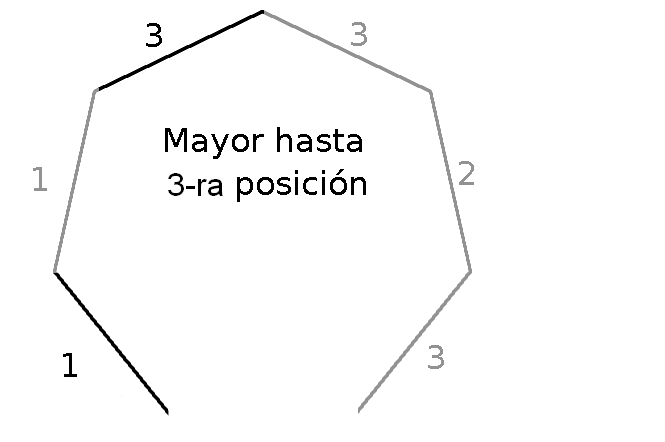
\includegraphics[width=0.3\textwidth]{imagenes/paso2b.PNG}}
\qquad
\subfloat{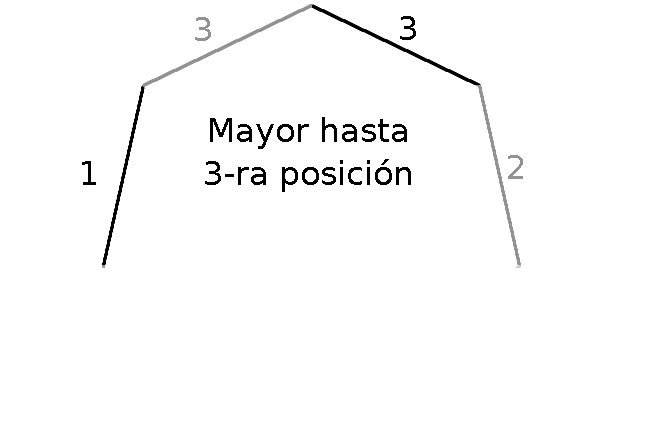
\includegraphics[width=0.3\textwidth]{imagenes/paso5a.png}}
\caption{Se calcula el matching máximo en los vectores - Tercer paso}
\end{figure}

\begin{figure}[H]
\centering
\subfloat{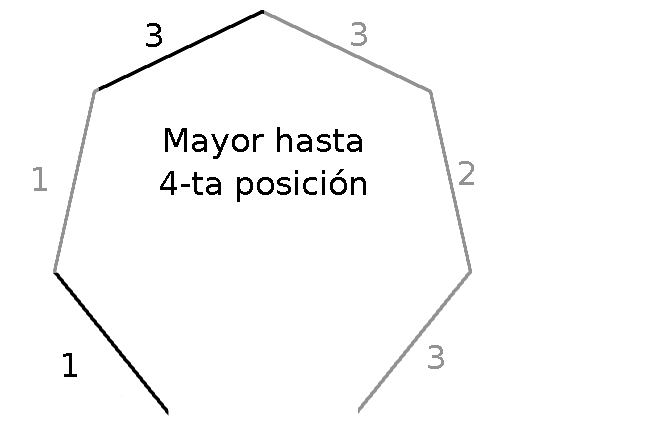
\includegraphics[width=0.3\textwidth]{imagenes/paso3b.png}}
\qquad
\subfloat{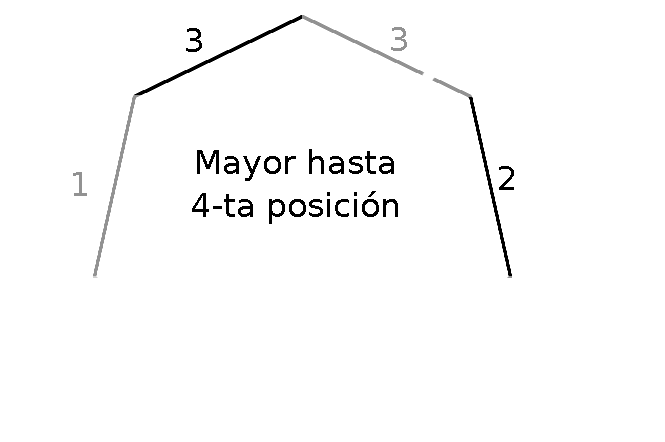
\includegraphics[width=0.3\textwidth]{imagenes/paso6a.png}}
\caption{Se finaliza un matching, se continúa el cálculo del otro}
\end{figure}

\begin{figure}[H]
\centering
\subfloat{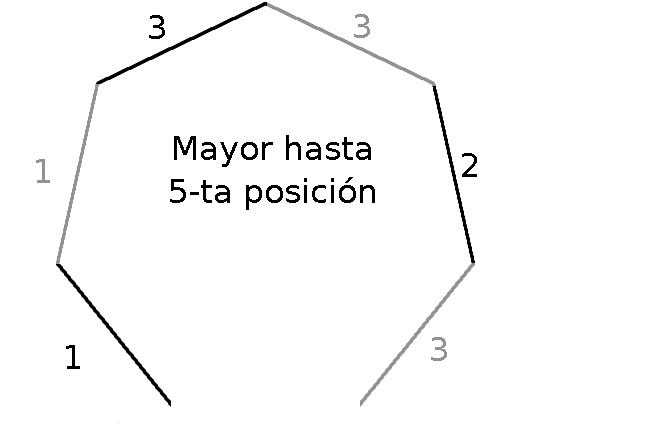
\includegraphics[width=0.3\textwidth]{imagenes/paso4b.png}}
\qquad
\subfloat{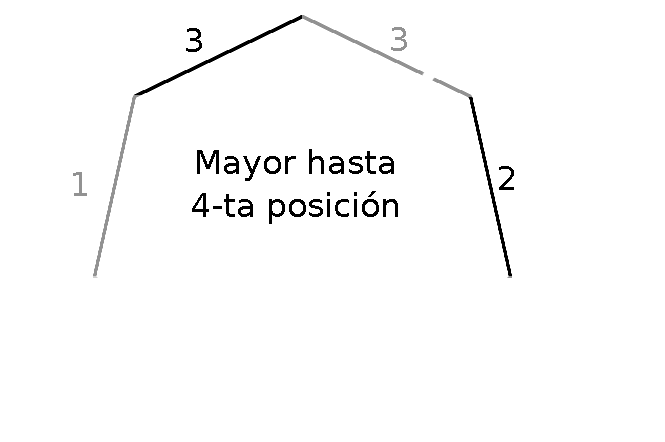
\includegraphics[width=0.3\textwidth]{imagenes/paso6a.png}}
\caption{Ante\'ultimo Paso}

\end{figure}

\begin{figure}[H]
\centering
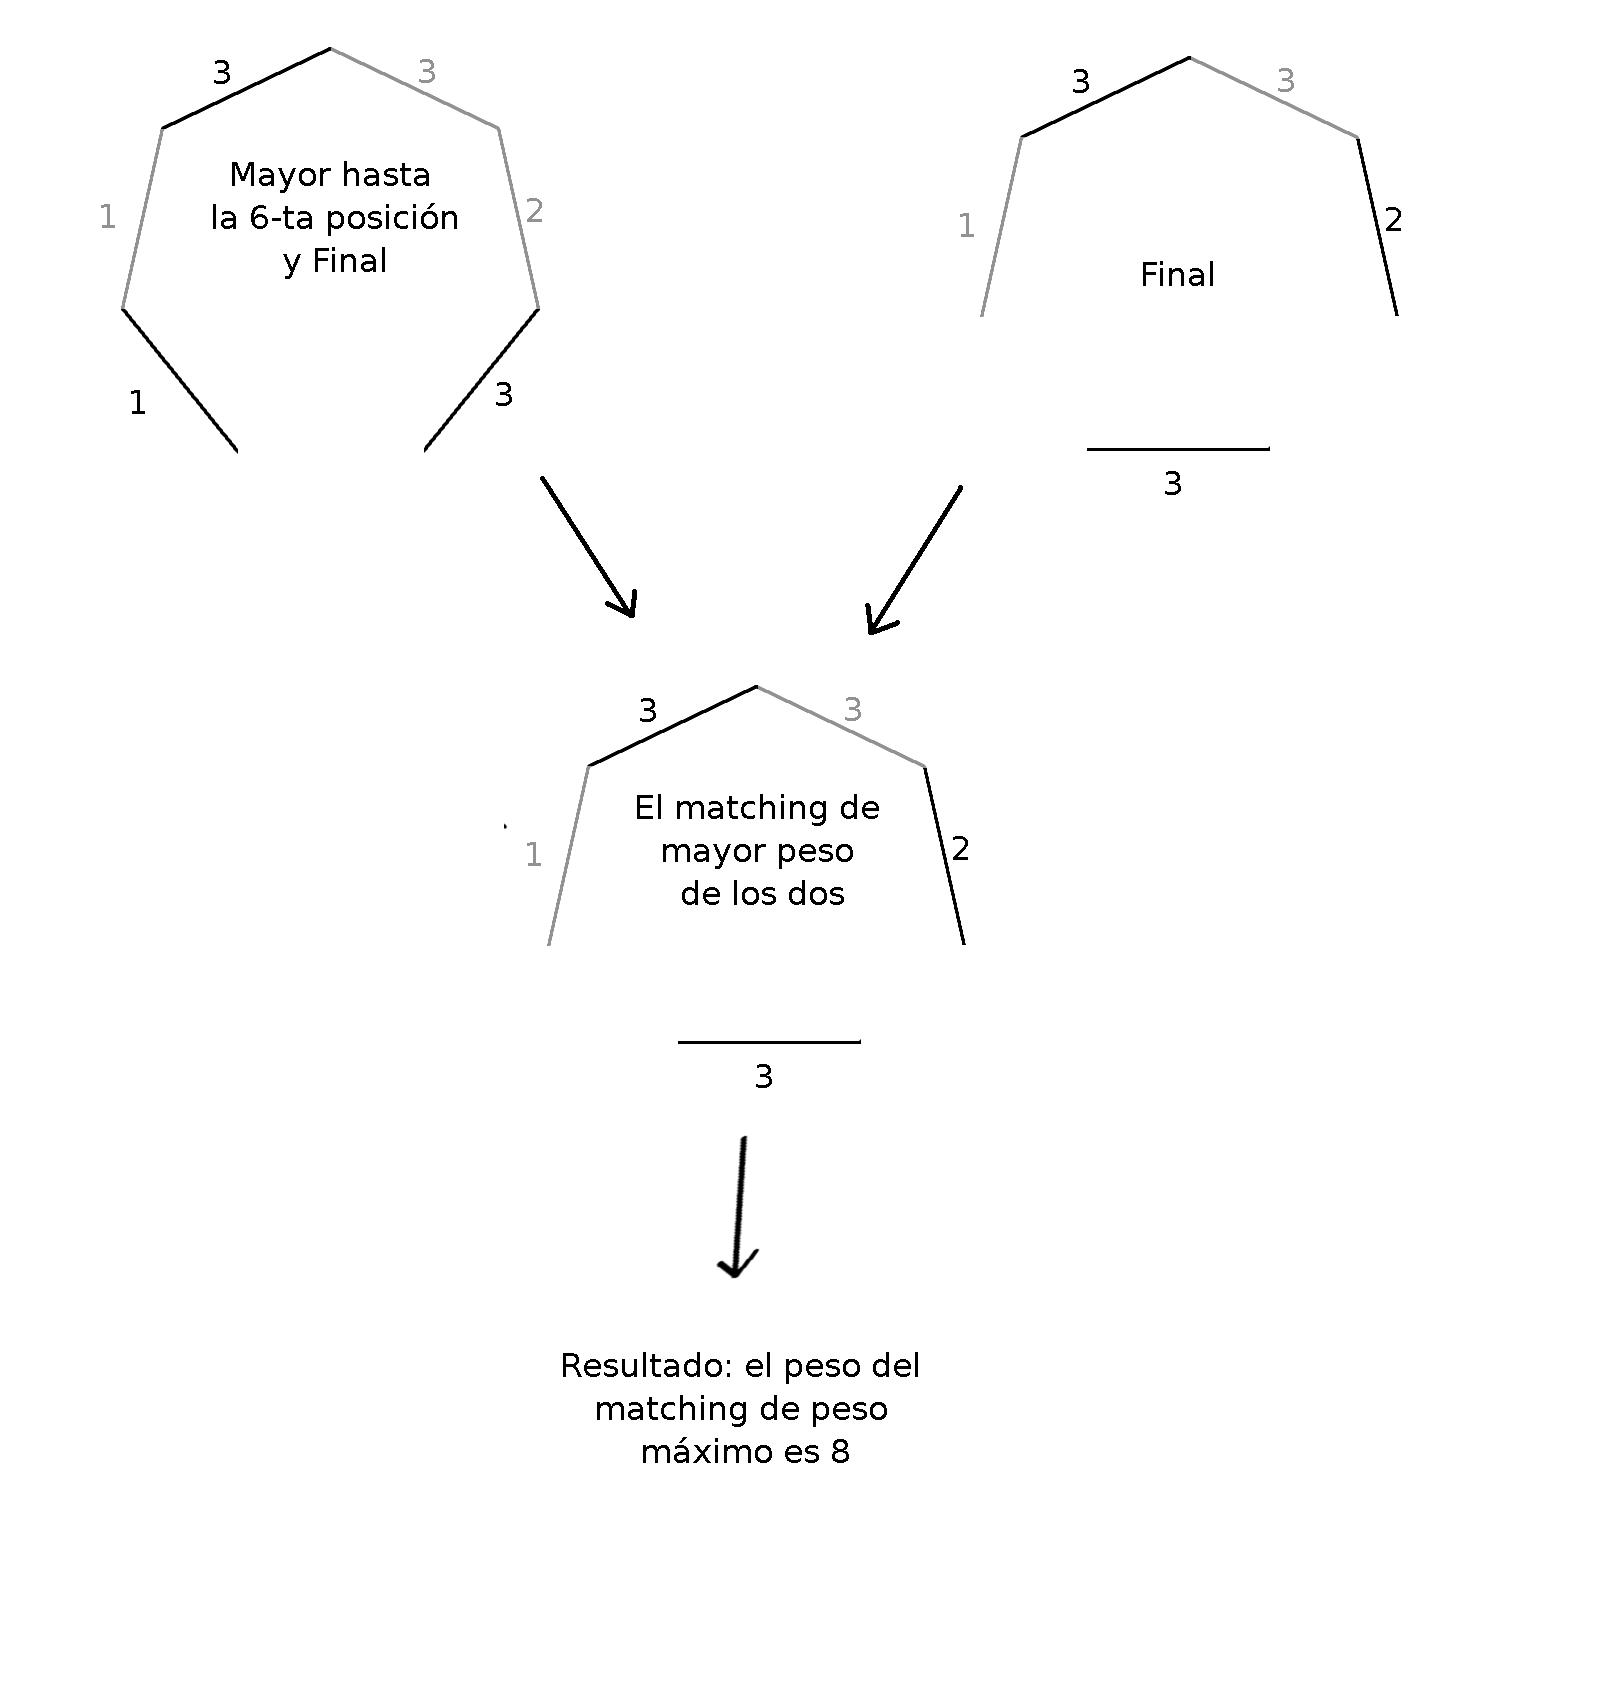
\includegraphics[width=0.7\textwidth]{imagenes/pasosFinales.png} 
\caption{Unión de los caminos}
\end{figure}

\subsection*{Demostración de correctitud}
\addcontentsline{toc}{subsection}{Demostración de correctitud} 

Sea S un matching de peso máximo para un camino $C =  C_1, C_2, ... , C_n $.
Se quiere demostrar que $peso(S) = max (peso( {C_n} \cup maxmatching(C_{1,n-2}) )$, 
peso( maxmatching$(C_{1,n-1}) ) ) $.

Para lo cual vamos a suponer que $S = maxmatching(C)$ y que $peso(S) \neq max(peso({C_n} \cup maxmatching(C_{1,n-2})) , peso(maxmatching(C_{1,n-1})))$. Peso(s) no puede ser menor ya que es un matching de peso máximo. Luego su peso es mayor.

 $ C_n \in S $, ya que si no fuera as\'i, entonces S es un matching de $C_{1,n-1}$, y por lo tanto el peso de S debe ser menor o igual al de $maxmatching(C_{1,n-1})$, pero supusimos que $peso(S) > peso(maxmatching(C_{1,n-1}))$. 


Como $ C_n \in S $, luego $ C_{n-1} \notin S$, luego  S - $C_n $ es un matching de $C_{1,n-2}$.


Como peso$({C_n} \cup$  maxmatching $(C_{1,n-2})) = peso(C_n) + peso(maxmatching(C_{1,n-2}))$
y $peso({C_n} \cup maxmatching(C_{1,n-2})) < peso(S)$, entonces $peso(maxmatching(C_{1,n-2})) < peso(S - {C_n})$, pero $S - {C_n}$ es un matching de $C_{1,n-2}$, por lo tanto $peso(S - {C_n}) \leq peso(maxmatching(C_{1,n-2}))$. LLegamos a un absurdo, producto de suponer que   $peso(S) \neq max(peso({C_n} \cup maxmatching(C_{1,n-2}), maxmatching(C_{1,n-1})) $.


\subsection*{Complejidad}
\addcontentsline{toc}{subsection}{Complejidad} 
Se analizará la complejidad de este algoritmo en función del modelo uniforme.

En primer lugar, el algoritmo dise\~{n}ado toma una arista cualquiera, lo cual se ejecuta en un tiempo constante dado que los vértices se encuentran en un vector de acceso indexado. Luego, se toman los dos vecinos que, dado que el grafo es un circuito simple, también se los puede obtener en un tiempo constante. Luego, el algoritmo realiza una llamada a otro algoritmo que resuelve el matching máximo sobre vectores. Por último, se realiza una comparación entre los dos resultados arrojados por la rutina auxiliar para poder devolver el máximo, siendo esta una operación también de costo constante. Es por esto que la complejidad de este algoritmo esta regida entonces por la complejidad de la rutina auxiliar a la que hace referencia, ya que todas las demás operaciones toman un tiempo constante de ejecución.

Resulta necesario ver entonces la complejidad del algoritmo de matching máximo sobre vectores.
Este algoritmo comienza realizando comparaciones del tama\~{n}o del vector para ver si el mismo se resuelve trivialmente. En todos estos casos los costos de las operaciones son constantes. Sin embargo, el peor caso, es que el vector pasado como parámetro contenga tres o más elementos, por lo que la complejidad del algoritmo estará dada por los costos de las operaciones en el caso de que el tama\~{n}o sea tres o más.

En este caso, lo primero que se realiza son dos asignaciones y una comparación, lo cual toma tiempo constante. Luego, se realiza un ciclo tomando valores desde tres hasta n. Una vez dentro del ciclo, se realizan varias operaciones de tiempo constante, más especificamente se realizan tres asignaciones, una suma y una comparación. Luego, al tener un ciclo que se ejecuta n-2 veces y sabiendo que dentro del ciclo las operaciones toman un tiempo constante, se puede aseverar que la ejecución de este ciclo será O(n). 

Por último, dado que en este último caso las operaciones son dos con tiempo constante y el ciclo mencionado, se puede asegurar que la complejidad total del algoritmo para encontrar el matching sobre un vector es O(n).

Finalmente, al ya haber mencionado que la complejidad del algoritmo principal se regía por la complejidad de la subrutina utilizada. Se puede ver que la complejidad de todo el algoritmo será lineal, es decir O(n). Es importante notar que para encontrar un matching máximo, como mínimo hay que observar todas las aristas, por lo que la complejidad lineal resulta ser óptima.



\subsection*{Análisis de resultados}
\addcontentsline{toc}{subsection}{Análisis de resultados} 

Para analizar este algoritmo, se basó el enfoque en dos aspectos diferentes. Por un lado, se encuentran los análisis sobre la correctitud de la solución propuesta y, por otro lado, se encuentra el análisis sobre el tiempo de ejecución para diferentes archivos de entrada, para poder realizar así, una correlación entre el tiempo de ejecución y la complejidad teórica calculada anteriormente.

\subsection*{Casos de correctitud}
\addcontentsline{toc}{subsection}{Casos de correctitud} 
Con el fin de realizar una comprobación empírica de la solución propuesta se generó un archivo de entrada con diez casos de prueba.
\begin{itemize}
\item Los primeros nueve casos de prueba, están conformados por los entregados por la cátedra, teniendo de esta manera las soluciones reales para contrastar con las arrojadas por el algoritmo.
\item El último caso de prueba esta conformado por un grafo de 30 aristas, con pesos de 1 a 30, ordenados consecutivamente. En este caso, se puede ver que el matching máximo está dado por tomar las aristas con valor par.
\end{itemize}

El análisis en este tipo de casos se basó solamente en la correctitud de los mismos y no en el tiempo de ejecución debido a que son grafos de tama\~{n}os muy peque\~{n}os y el tiempo de ejecución no sobrepasa los 2 microsegundos en ninguno de los casos.

Para todos los casos propuestos los resultados fueron satisfactorios al ser contrastados con la soluciones previamente obtenidas.

\subsection*{Casos para probar el tiempo de ejecución}
\addcontentsline{toc}{subsection}{Casos para probar el tiempo de ejecución} 
Para poder analizar cómo se comporta el algoritmo en función del tama\~{n}o del grafo a procesar, se implemento un generador de ciclos simples al azar. El mismo se realizó para que arrojase una salida con 500 grafos diferentes, el primero con 10000 aristas, el segundo con 10500 y así sucesivamente. Una vez obtenidos los tiempos de ejecución de cada uno de estos casos, se procedió a graficar los resultados para poder contrastar con la complejidad obtenida teóricamente.

A continuación se presenta un gráfico donde se encuentran simultaneamente los datos obtenidos y un ajuste lineal de los mismos.


\begin{figure}[H]
\centering
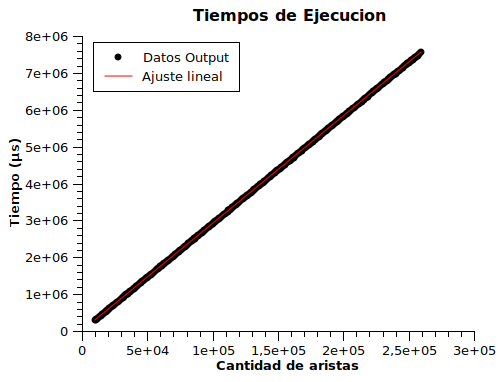
\includegraphics[width=0.7\textwidth]{imagenes/Resultados1.png} 
\caption{Gráfico 1}
\end{figure}

Como se puede observar en el gráfico, los resultados fueron satisfactorios. El ajuste lineal arrojó un coeficiente de correlación de aproximadamente 0.99999, mostrando empíricamente que la complejidad teórica calculada se condice con los tiempos reales de ejecución. 

\subsection*{Conclusiones}
\addcontentsline{toc}{subsection}{Conclusiones} 

Luego de obtener los resultados para el presente ejercicio, se concluyen varios puntos importantes:

\begin{itemize}
\item Si bien el problema de matching es de gran complejidad algorítmica, es necesario explotar el hecho de que sólo se debe realizar sobre ciclos simples. El hecho de haber explotado esta característica de los grafos presentes en la entrada del algoritmo, fue de gran importancia al momento de lograr un algoritmo eficiente que sólo recorriese cada arista una única vez.
\item Resulta de gran importancia pensar diferentes variantes para el algoritmo con el fin de encontrar la versión más eficiente. Durante el dise\~{n}o del algoritmo se pensó tanto una estrategia de divide and conquer, como una estrategia de programación dinámica. Si bien ambas resolvían el problema satisfactoriamente dado que la idea era básicamente la misma sólo que se invertía el orden del recorrido del grafo, cabe destacar como la simple mejora de recorrer desde el primer elemento hasta el último trajo la gran ventaja de preguntar por cada configuración de aristas una sola vez, generando así un algoritmo de orden lineal, a diferencia del algoritmo exponencial obtenido por divide and conquer.
\item La complejidad teórica calculada se pudo ver reflejada en los casos de prueba propuestos. Se cree que la calidad del ajuste lineal que se consiguió se debió a que el algoritmo no presenta mejores o peores casos; es decir, para todo grafo posible el algoritmo debe recorrer exactamente la misma cantidad de veces cada arista. De esta manera, los casos de prueba creados aleatoriamente no pueden ser beneficiados por el azar en ningún caso, generando una casi perfecta correlación lineal en función de la cantidad de aristas.
\end{itemize}



\begin{center}
\item \section*{Ejercicio 2: Se inunda la isla}
\addcontentsline{toc}{section}{Ejercicio 2: Se inunda la isla} 

\end{center}

\subsection*{Introducción}
\addcontentsline{toc}{subsection}{Introducción}

En este ejercicio se pedía encontrar el área que no se inunde en una isla plana luego de ciertas condiciones.

En primer lugar, se tiene una isla que posee la misma altura en todos sus puntos, es por esto que si la marea sube la isla se inunda por completo. La solución para que las partes importantes de la isla no se inunden cuando sube la marea, es poner una serie de vallas rectangulares que no dejen pasar el agua hasta cierta altura. La idea sería entonces, colocando adecuadamente estas vallas, encerrar partes de la isla para que el agua no pueda entrar.

El problema consiste en, dado un conjunto de vallas y el nivel de la marea, calcular cuál es el área de la isla que no va a ser inundada.

\subsection*{Algoritmo}
\addcontentsline{toc}{subsection}{Algoritmo}

A continuación se presenta una explicación al algoritmo propuesto como solución, seguido por su respectivo pseudocódigo.

En primer lugar se observa que, por restricción del problema, las vallas no pueden estar en cualquier lado, sino que su coordenada (x,y) del punto inferior izquierdo esta formada por x e y enteros. Asimismo, como la longitud de una valla también es entera, la coordenada del vértice restante también será entera. De esta manera, podemos ver que la isla se puede pensar como una grilla de cuadrados de 1x1. Luego, esta grilla fue pensada como un grafo, donde cada cuadrado de la grilla es un nodo y las aristas están dadas por la relación entre un cuadrado y sus 4 posibles vecinos. Para armar esta grilla, se calcularon los mínimos y máximos valores de las vallas (como se ve en la siguiente figura) en x y en y, ya que por fuera de estos los cuadrados que pertenezcan a la isla se inundarán de todos modos (ya que no hay vallas que los cubran).


\begin{figure}[H]
\centering
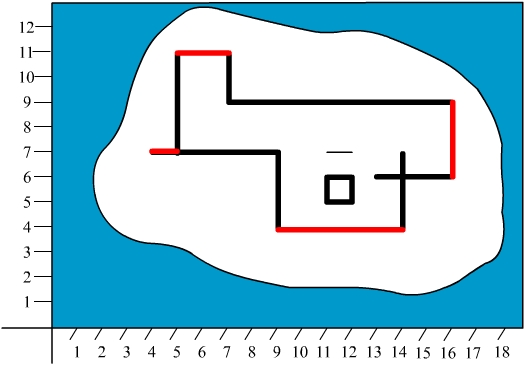
\includegraphics[width=0.5\textwidth]{imagenes/im2_ej2.jpg} 
\caption{Detecci\'on de m\'aximos y m\'inimos}
\end{figure}

Al comenzar el algoritmo, todos los cuadrados están relacionados con sus vecinos con aristas de peso 0. Esto quiere decir que si un cuadrado se inunda, los cuadrados que estén relacionados con ese por una arista de peso 0 también se van a inundar. 

Luego, se recorren todas las vallas dadas por el problema y se setean las nuevas relaciones entre los cuadrados, es decir, si existe una valla de altura 4 entre el nodo $v_1$ y el nodo $v_2$, lo que se hace es ponerle un peso de 4 a la arista que los relaciona. Indicando así que solamente si la marea es mayor a 4, el agua pasará de ese $v_1$ a $v_2$ directamente.

Por último, lo que se hace es crear una circunvalación de nodos que se inundan alrededor del grafo real como lo muestra la siguiente figura.

\begin{figure}[H]
\centering
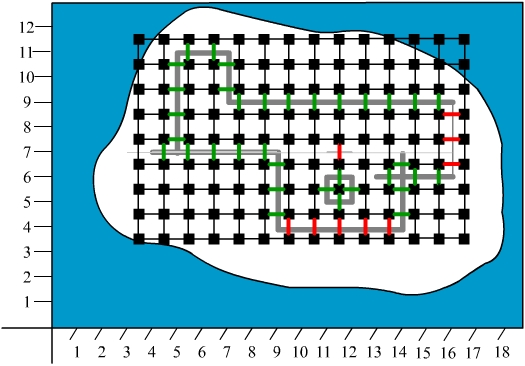
\includegraphics[width=0.5\textwidth]{imagenes/im3_ej2.jpg} 
\caption{Generaci\'on del grafo}
\end{figure}

Se realiza BFS desde uno de los nodos de la circunvalación (que seguro se inunda, por estar por fuera de las vallas) y se cuenta cuántos nodos tiene la componente conexa que el BFS recorre por completo. Cabe destacar que dicho BFS toma que un nodo es vecino de otro si la arista que los une tiene peso menor a la marea, si no, se puede decir que la valla es efectiva entre esos dos nodos y no hay inundación de uno hacia el otro. Una vez obtenida la cantidad total de nodos dados por el recorrido en anchura, resta el último paso que es realizar la sustracción entre los nodos totales de la grilla, y los nodos inundados; obteniendo así, la cantidad total de nodos que no fueron inundados gracias a la protección de las vallas. Por último, como cada nodo representa un cuadrado de área 1, la cantidad de nodos no alcanzados por el BFS es igual al área no inundada.

A continuación se presenta el pseudocódigo del algoritmo recientemente explicado.

\begin{verbatim}
areaNoInundada(){

        vector vallas;
        leer(vallas)
        maxmin(vallas)
        matriz nodo[alto][ancho];
        seteamosMatriz(matriz)
        int inundadas  <- bfsContador(matriz)
        return (ancho*alto - inundadas)
}
\end{verbatim}



\begin{itemize}
\item leer(vallas): Carga en el vector vallas todas las provenientes del input.

\item maxmin(vallas): Setea ciertas variables con el tama\~no máximo que tendrá la isla delimitada por las vallas más externas.

\item seteamosMatriz(matriz): Usando las variables seteadas por maxmin crea un grafo (representado con una matriz) donde establece 4 relaciones por nodo (con sus vecinos) donde el peso de la arista es la altura de la valla que debe atravesar.

\item bfsContador(matriz): Recorre el grafo usando bfs, por cada nodo que visita suma uno a una variable que al final devuelve. Recorre todos los nodos que se inundan dado que son los que se relacionan (si la marea supera el peso de las aristas). De este modo al finalizar obtenemos cuántos nodos visitamos coincidiendo con cuántos nodos se inundan.
\end{itemize}

A continuaci\'on se presenta un seguimiento paso a paso del algoritmo, una vez ya conseguidos los m\'aximos y m\'inimos.

\begin{figure}[H]
\centering
\subfloat[Grafo vacio]{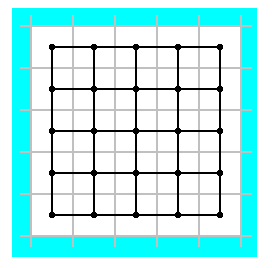
\includegraphics[width=0.3\textwidth]{imagenes/grafSinVallas.png}}
\qquad
\subfloat[Grafo con vallas]{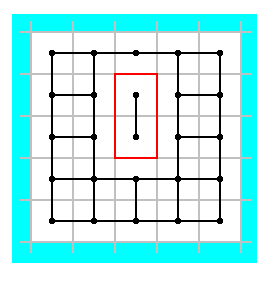
\includegraphics[width=0.3\textwidth]{imagenes/grafConVallas.png}}
\caption{Isla vacia y posicionamiento de las vallas}
\end{figure}

\begin{figure}[H]
\centering
\subfloat[Primer Paso]{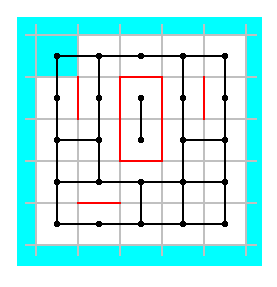
\includegraphics[width=0.2\textwidth]{imagenes/inundPaso1.png}}
\qquad
\subfloat[Segundo Paso]{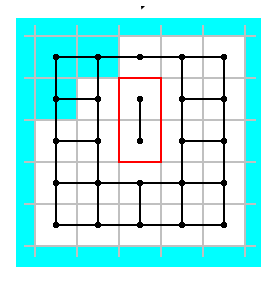
\includegraphics[width=0.2\textwidth]{imagenes/inundPaso2.png}}
\qquad
\subfloat[Tercer paso]{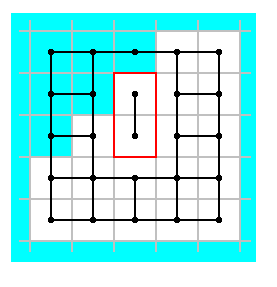
\includegraphics[width=0.2\textwidth]{imagenes/inundPaso3.png}}
\caption{BFS}
\end{figure}

\begin{figure}[H]
\centering
\subfloat[Cuarto Paso]{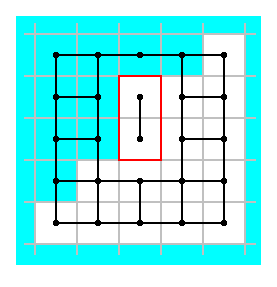
\includegraphics[width=0.2\textwidth]{imagenes/inundPaso4.png}}
\qquad
\subfloat[Quinto Paso]{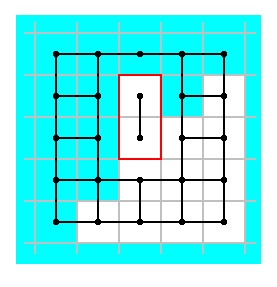
\includegraphics[width=0.2\textwidth]{imagenes/inundPaso5.png}}
\qquad
\subfloat[Sexto Paso]{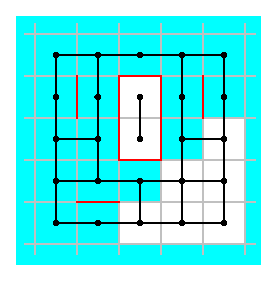
\includegraphics[width=0.2\textwidth]{imagenes/inundPaso6.png}}
\caption{BFS}
\end{figure}

\begin{figure}[H]
\centering
\subfloat[S\'eptimo Paso]{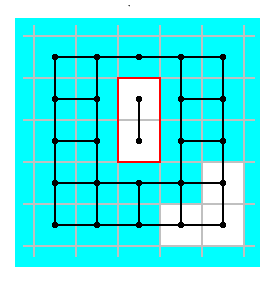
\includegraphics[width=0.2\textwidth]{imagenes/inundPaso7.png}}
\qquad
\subfloat[Octavo Paso]{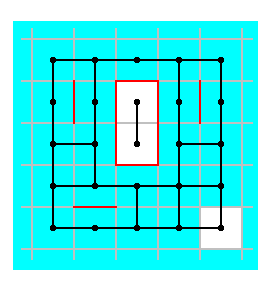
\includegraphics[width=0.2\textwidth]{imagenes/inundPaso8.png}}
\qquad
\subfloat[\'Ultimo Paso y cuenta final]{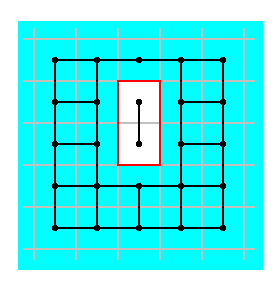
\includegraphics[width=0.2\textwidth]{imagenes/inundPasoFinal.png}}
\caption{Fin del BFS}
\end{figure}


\subsection*{Complejidad}
\addcontentsline{toc}{subsection}{Complejidad}
Para analizar la complejidad se utilizó el modelo uniforme. En este modelo el análisis no está centrado en el tama\~{n}o de los operandos, por lo que el tiempo de ejecución de cada operación se considera constante.

Si tomamos como tama\~no de entrada la cantidad de vallas (CV en adelante), y como sabemos que estas no se solapan en más de un punto, podemos acotar por arriba a la cantidad de vallas, por un múltiplo de la cantidad de nodos, si bien acotar las vallas por cuatro veces la cantidad de nodos resulta una cota grosera ya que se están contando muchas vallas varias veces, la cota resulta útil para poder enfocar el análisis del algoritmo simplemente a la cantidad total de nodos; es decir, a la cantidad de casillas en la cuadrícula.

En primer lugar, la función maxmin, busca máximos y mínimos linealmente en un vector de vallas, por lo cual es de orden O(CV) ya que se recorre todo el vector de vallas una vez.

En segundo lugar, se realiza la asignaci\'on de toda la matriz mediante la información entregada por las vallas, en esta rutina se itera sobre todas las vallas y se asignan las relaciones entre los nodos a partir de las alturas de las vallas pasadas como parámetro. En el peor de los casos, se tienen que asignar las cuatro relaciones para cada uno de los nodos de la grilla. Como acceder al nodo se realiza en tiempo constante, y luego hacer los cuatros posibles cambios también se realiza en tiempo constante, esta rutina posee una complejidad de O(n) siendo n la cantidad de nodos de la grilla, ya que se realiza un ciclo sobre todos ellos, mientras que en cada iteración se realizan operaciones de complejidad O(1).

En último lugar, lo que se hace es realizar un BFS para lograr identificar la cantidad de nodos de la componente conexa que se inunda. La rutina de BFS tiene una complejidad de O(n+m) siendo n la cantidad de nodos del grafo, y m la cantidad de aristas del mismo. Sin embargo, en este caso podemos acotar m por 2*n, ya que en el peor de los casos, cada nodo posee 4 vecinos. Luego, la complejidad de BFS en este caso es O(n).

En resumen, se realizan tres rutinas, la primera tiene una complejidad O(CV) que ya se mencionó que se puede acotar por O(n); luego, se realizan otras dos rutinas que ambas tiene complejidad O(n). Entonces, la complejidad total del algoritmo, es O(n), siendo n la cantidad de nodos del grafo que representa la isla. Cabe destacar que esta complejidad es análoga a O(S), siendo S el área del rectángulo donde se puede inscribir la isla, ya que si bien el algoritmo agrega una fila y una columna O((altura+2)*(ancho+2)) = O(altura*ancho) = O(S).

\subsection*{Análisis de resultados}
\addcontentsline{toc}{subsection}{Análisis de resultados}
Para analizar el funcionamiento del algoritmo propuesto como solución del problema, se realizaron dos tipos diferentes de casos de pruebas. Por un lado, se intentó probar la correctitud del algoritmo mediante algunos casos de prueba de tama\~{n}o considerablemente peque\~{n}o, con el objetivo de poder contrastar las soluciones arrojadas por el algoritmo con las soluciones que se obtienen manualmente al poder visualizar la isla con las vallas que corresponden. Por otro lado, se intentó contrastar la complejidad teórica con el comportamiento real del algoritmo creando varias instancias de tama\~{n}os considerablemente grandes.

\subsection*{Casos de Correctitud}
\addcontentsline{toc}{subsection}{Casos de Correctitud}
Para analizar la correctitud del algoritmo, se utilizaron los siguientes casos de prueba:
\begin{itemize}
\item En primer lugar, se utilizaron los casos de prueba entregados por la cátedra. Los mismos constan de 6 islas con diferentes configuraciones de vallas.
\item Por otro lado, se generaron 9 islas también con diferentes configuraciones de las vallas, de manera que los resultados de las mismas se pudiesen verificar manualmente.
\end{itemize}

Cabe destacar que todos los resultados obtenidos se contrastaron satisfactoriamente con los resultados esperados, tantos los entregados por la cátedra, como los obtenidos manualmente.

En este tipo de casos, solamente se menciona cómo fue el comportamiento del algoritmo en cuanto a la correctitud y no en cuanto al tiempo de ejecución debido a que, en primer lugar, los tama\~{n}os de los grafos que represetan las islas son muy chicos como para obtener tiempos de ejecución representativos; y, por otro lado, las islas utilizadas poseen diferentes números de vallas, lo que traería fluctuaciones en los tiempos de ejecución en caso de querer ser analizados.

\subsection*{Casos para probar el tiempo de ejecución}
\addcontentsline{toc}{subsection}{Casos para probar el tiempo de ejecución}
Como se explicó en la sección correspondiente, la complejidad de este algoritmo es lineal respecto de la cantidad de nodos del grafo que representa al rectángulo que inscribe a la isla. Es por esto que, para poder ver la relación entre la complejidad teórica y el comportamiento real del algoritmo, se crearon varias instancias de diferentes islas donde la cantidad de nodos creciera linealmente.

Se crearon 500 casos de prueba donde se mantuvieron ciertas características invariantes para poder crear instancias comparables, mientras que el único parámetro que se varió fue la altura total del rectángulo en cuestión.
Los casos de prueba se realizaron de la siguiente manera:
\begin{itemize}
\item Todos los casos tienen la marea de nivel 3.
\item Todos los casos poseen 8 vallas en total, todas de altura 4. Cuatro de las vallas se encuentran dentro del rectángulo encerrando un área no inundable de 1*2, con el simple objetivo de poseer un área no inundable.
\item De las otras 4 vallas, 3 son fijas, delimitando el ancho del rectángulo desde x igual a 1 hasta x igual a 10 y la restante delimita el borde inferior en y igual a 1.
\item La valla restante es la que se va modificando para generar instancias cada vez más grandes. Comienza en el primer caso delimitando el borde superior en y igual a 10000, y luego va subiendo este límite 500 unidades por cada caso.
\end{itemize}

Por lo explicado anteriormente, se puede ver que las islas son todas muy parecidas excepto por la cantidad de nodos en total que varían desde 100000, subiendo de a 5000 nodos por cada caso. La idea de realizar islas muy parecidas excepto por la cantidad de nodos, fue que el seteo de vallas y sus respectivas relaciones fueran análogas para todos los casos y que no fueran factor de fluctuaciones no deseadas en los tiempos de ejecución.

A continuación se presenta un gráfico donde se encuentran plasmados los tiempos de ejecución en cada caso, en función de la cantidad de nodos del grafo correspondiente.

\begin{figure}[H]
\centering
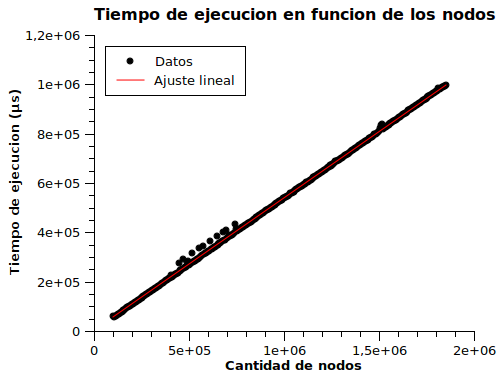
\includegraphics[width=0.7\textwidth]{imagenes/Resultados2.png} 
\caption{Gráfico 1}
\end{figure}


Como se puede observar, las observaciones empíricas de cómo funciona el algoritmo se condicen con la complejidad teórica
calculada anteriormente. Si bien se denota la presencia de algunos \emph{outliers}, también se puede observar claramente
como los datos están relacionados por una función lineal tal como la complejidad teórica predicaba. Al realizar el ajuste lineal
se consiguió un ajuste con un coeficiente de correlación de aproximadamente 0.999.

\subsection*{Conclusiones}
\addcontentsline{toc}{subsection}{Conclusiones}
Luego de obtener los resultados pertinentes a los diferentes casos de prueba se concluye que:
\begin{itemize}
\item Es importante tener en cuenta varios modelos diferentes a la hora de dise\~{n}ar un algoritmo para resolver un problema
en particular, ya que si bien la idea de una inundación de una isla puede estar bastante alejada de un problema de grafos, lograr
esta correlación hizo que el problema se pudiese realizar con un buen orden de complejidad y minimizando bastante bien la cantidad de 
veces que se itera sobre las diferentes partes de la isla.
\item Resulta de gran importancia tener en cuenta algunos peque\~{n}os detalles de dise\~{n}o, ya que estos pueden ser muy
relevantes en el resultado final. Por ejemplo, en este algoritmo fue importante el hecho de agrandar la grilla una linea en cada dirección, si bien la complejidad del mismo no hubiese cambiado, se tendr\'ian que haber hechos varios BFS, generando un algoritmo un poco m\'as engorroso.
\item La complejidad teórica calculada se pudo contrastar empíricamente con los casos de prueba utilizados. Igualmente, 
cabe destacar que se presentaron algunos pocos outliers que se desconoce su origen, para todos los demás datos, se puede ver que
el tiempo de ejecución aumenta de manera lineal en función de la cantidad de nodos.
\item Para poder analizar el tiempo de ejecución fue necesario buscar casos de prueba donde lo único que variase fuera la cantidad de nodos,
si otro parámetro hubiese variado (la cantidad de vallas por ejemplo, o la disposición de las mismas) el tiempo de ejecución 
podría haber fluctuado, ya que sin tener una relación con la cantidad de nodos dicha fluctuación tendr\'ia un efecto que no es deseado. 
\end{itemize}


\begin{center}
\item \section*{Ejercicio 3: Bernardo Armando Pandillas}
\addcontentsline{toc}{section}{Ejercicio 3: Bernardo Armando Pandillas}

\end{center}

\subsection*{Introducción}
\addcontentsline{toc}{subsection}{Introducción}


En este problema lo que se quiere es, teniendo un conjunto de personas y sabiendo si se conocen entre sí, armar dos grupos de tres personas cada uno, un grupo en el cual las 3 personas se conozcan mutuamente, y otro grupo en el cual ninguno esté relacionado con otro.


En el caso que se puedan armar varios grupos con las restricciones planteadas, los que se deben encontrar son los menores lexicográficamente, para cada uno de los dos casos. Es decir, si se representa cada grupo con una terna ordenada ascendentemente, la terna que se busca será menor que cualquier otra terna que represente a un grupo válido.

Se considera que una terna es menor que otra si la primera componente de la primera terna es menor, o si es igual y la segunda de la misma es menor, o si tanto la primera como la segunda son iguales y la tercera es menor, en cada caso con respecto a la misma componente de la otra terna.
\begin{displaymath}
\left(a, b, c \right) < \left( d, e, f\right) \Leftrightarrow 
\left( a < d \right) \vee \left( a = d \wedge b < e \right) \vee \left( a = d \wedge b = e \wedge c < f \right)
\end{displaymath}


\subsection*{Algoritmo}
\addcontentsline{toc}{subsection}{Algoritmo}

Para lograr el objetivo deseado se opt\'o por representar el problema utilizando un grafo en donde cada vértice del mismo representase a una persona diferente, mientras que las aristas fuesen las encargadas de representar las relaciones de conocimiento, teniendo así la presencia de una arista entre dos nodos diferentes si y solo si las personas representadas por dichos nodos se conocen.


Una vez obtenido el grafo de relación, lo que se busca es un clique de 3 nodos, ya que se puede ver que existe un clique de tres nodos si y sólo si las personas representadas por los nodos que estén en dicho clique se conocen todas entre sí\footnote{Ver Apéndice \ref{dem_clique}}.


Encontrar un clique de 3 nodos, encontraría entonces las conformaciones posibles para el grupo Coppersmith. Luego, se necesita buscar como formar el grupo Winograd. Para encontrar este grupo de tres personas que no se conozcan entre sí, lo que se hizo fue resolver el mismo problema pero en el grafo complemento, ya que este nuevo grafo representa las no-relaciones entre las personas\footnote{Ver Apéndice \ref{dem_clique}}.

Una vez demostrado que la extrapolación del modelo elegido es correcta para poder resolver el problema pedido, se aboca el algoritmo a encontrar un clique de tres nodos en el grafo.
Para encontrar el clique se realizan los siguiente pasos:

\begin{enumerate}
\item En primer lugar, se confecciona la matriz de adyacencias utilizando las relaciones entre las personas, en la cual el nodo i-ésimo representa a la i-ésima persona. A partir de aquí, se llamará $A$ a esta matriz de adyacencia.
\item Luego, sea $C = A^3$, entonces se puede ver que $C$ tiene en la i-ésima posición de su diagonal la cantidad de caminos de longitud 3 desde el nodo i hasta el nodo i. \footnote{Teórica Algoritmos III} Esto justamente indica la presencia de un clique de 3 nodos dado que, en el caso especial de 3 nodos, un clique o un circuito es lo mismo.
\item Una vez que se tiene la matriz elevada al cubo, se puede conocer los nodos que están en un circuito de 3 nodos mirando la diagonal. Se busca en $C$ el mínimo i tal que $C_{i,i} \neq 0$, llamémoslo j. Si existe, entonces, el menor clique de 3 nodos contendrá a j. Si no fuera así, entonces existe $k < j$ tal que $C_{k,k} \neq 0$, lo cual es un absurdo, ya que j es el mínimo i tal que $C_{i,i} \neq 0$. Si no existe, termina el algoritmo indicando que como no hay ninguna persona que esté involucrada en un ciclo de 3 nodos, entonces no se puede armar el grupo Coppersmith.
\item Una vez obtenido el menor nodo que está presente en un clique de 3 nodos, de todas las combinaciones posibles para los otros dos nodos, se elige la menor tal que los tres nodos forman un clique. En la implementación se optimiza esta última selección, evitando generar combinaciones que se sepa anticipadamente que no corresponden a un clique. De esta manera se obtuvo el grupo de tres personas que se conocen entre sí.
\item Por último se obtiene el grafo complemento de $G$, y se realizan las mismas operaciones para obtener el grupo de tres personas que no se conocen entre sí, el grupo Winograd.
\end{enumerate}

\subsection*{Complejidad}
\addcontentsline{toc}{subsection}{Complejidad}

Para analizar la complejidad del algoritmo, se va ir analizando qué se hace en cada paso, calculando la complejidad del mismo.

En primer lugar, se setea toda la matriz de adyacencias mediante la información obtenida del caso pertinente. Lo que se hace es ir poniendo en cada posición un 0 o un 1 según corresponda, es por esto que este paso es del orden de $n^2$, siendo $n$ la cantidad de nodos del grafo.

Luego, se obtiene $C = A^3$ utilizando el algoritmo de Strassen para realizar el producto de matrices. La cantidad de operaciones que realiza este algoritmo está en $O\left(m^{log_2\left(7\right)}\right)$, para una matriz de $m$ filas y $m$ columnas.\footnote{Ver Referencia Bibliogr\'afica 1.} En el caso de que el grafo tenga $n$ nodos, es necesario generar una matriz de $m \times m$, con $m \leq 2n$, ya que es necesario que $m$ sea una potencia de dos. De esta forma, la cantidad de operaciones para realizar el producto de matrices está en $O\left(7 \times \left(n ^{log_2 \left( 7\right)} \right) \right) = O\left(n^{log_2\left(7\right)}\right)$.



Una vez obtenida la matriz elevada al cubo, es momento de buscar el mínimo elemento de la diagonal que sea distinto de 0. Se puede encontrar en $C$ el mínimo $i$ tal que $C_{i,i} \neq 0$ en $O\left(n\right)$ operaciones, ya que para cada posición de la diagonal se realiza una cantidad constante de operaciones para verificar si en dicha posición hay un cero. Para realizar esto, se recorre toda la diagonal que posee n elementos, cumpliendo así con la complejidad dicha.

Luego de obtener el menor nodo que se encuentra en un clique, hay que generar todas las demás combinaciones para ver cuales forman un clique. 
Al generar todas las combinaciones de dos nodos la cantidad de operaciones para obtener la menor está en $O\left(n^2\right)$, ya que se requiere una cantidad constante de operaciones para generar cada combinación, verificar si es un clique y compararla con la menor hasta el momento.

Luego, al tener todos los cálculos realizados para la busqueda del grupo Coppersmith, se puede ver por todo lo antedicho que la operación predominante esta dada por la multiplicación de las matrices que se realiza en $O\left(n^{log_2\left(7\right)}\right)$, siendo esta la complejidad del algoritmo para toda esta primer parte.

Por último se realizan las mismas operaciones sobre el grafo complemento. Para lo cual se invierte la matriz de adyacencias en $O \left( n^2 \right)$.


Entonces, como se puede ver, la complejidad computacional del algoritmo en el modelo uniforme está dada por las operaciones correspondientes a la multiplicación de matrices, en $O \left( n^{log_2\left(7\right)} \right) $, ya que el resto del algoritmo tiene un orden menor. Como $log_2\left(7\right) < 2.9 $, el algoritmo realiza una cantidad de operaciones de un orden estrictamente menor a $O\left( n^3\right) $.




\subsection*{Análisis de resultados}
\addcontentsline{toc}{subsection}{Análisis de resultados}
Para analizar el funcionamiento del algoritmo propuesto como soluci\'on del problema, se realizaron dos tipos de pruebas. Pruebas de correctitud, es decir tomar instancias chicas donde se conociese como deber\'ia ser la conformaci\'on de los dos grupos, para luego constrastarlo con los resultados del algoritmo; y, por otro lado, pruebas para poder visualizar emp\'iricamente el tiempo de ejecuci\'on del algoritmo.

\subsection*{Casos de Correctitud}
\addcontentsline{toc}{subsection}{Casos de Correctitud}
En este apartado, se centr\'o el estudio, en poder constratar con instancias conocidas el resultado del algoritmo Para esto, se realizaron los casos de prueba basados en los entregados por la c\'atedra. De esta manera, se pudo comparar los resultados que imprimio el algoritmo, con los resultados tambi\'en entregados por la c\'atedra. En todos los casos, la comparaci\'on fue satisfactoria. 

Cabe destacar que los casos utilizados para visualizar el tiempo de ejecuci\'on, explicados en la siguiente secci\'on, tambi\'en conformaron pruebas para la correctitud, ya que en los mismos las conformaciones de los dos grupos se podia ver manualmente aunque se tratasen de grupos numerosos.

Por \'ultimo, se destaca que para estos casos no se presentan gr\'aficos ya que los tiempos de corrida de los mismos no result\'o relevante, sino solamente su correctitud.

\subsection*{Casos para probar el tiempo de ejecuci\'on}
\addcontentsline{toc}{subsection}{Casos para probar el tiempo de ejecuci\'on}

En esta secci\'on lo que se busc\'o fue generar varios casos de prueba que lograsen mostrar cuanto tarda el algoritmo para poder constratar estos resultados con la complejidad te\'orica calculada anteriormente. Para realizar esto, se generaron varios casos de pruebas con la siguientes caracter\'isticas:

\begin{itemize}
\item Los casos analizados contienen grupos de 32 a 680 personas.
\item Todos los casos contienen las mismas relaciones, las unicas relaciones de conocimiento que existen son entre la persona 1 y la 2, entre la persona 1 y la 3 y entre la persona 2 y la 3. De esta manera, los grupos conformados en todos los casos son los mismos.
\item Por lo dicho anteriormente, todos los casos deber\'ian tener diferencia en el tiempo de ejecuci\'on en la multiplicaci\'on de matrices, ya que luego los grupos se encuentran rapidamente y para todos por igual.
\end{itemize}
A continuaci\'on se presentan dos gr\'aficos con los tiempos obtenidos en las corridas, en primer lugar se muestran todos los casos, y luego se muestran los que solamente involucran potencias de dos en la cantidad de personas.

\begin{figure}[H]
\centering
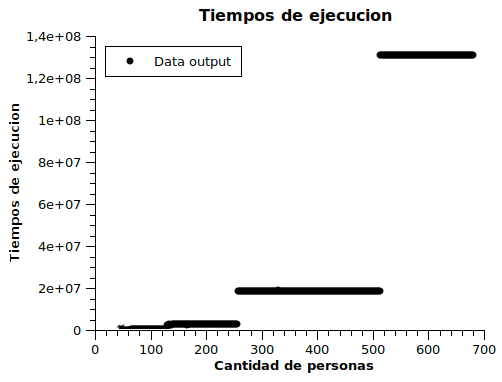
\includegraphics[width=0.7\textwidth]{imagenes/Resultados3.png} 
\caption{Gráfico 1}
\end{figure}

\begin{figure}[H]
\centering
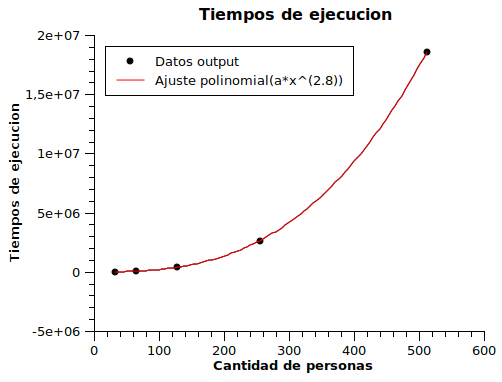
\includegraphics[width=0.7\textwidth]{imagenes/Resultados3Potencias2.png} 
\caption{Gráfico 2}
\end{figure}



Como se puede ver en el gr\'afico, los resultados arrojados se condicen con el an\'alisis te\'orico realizado anteriormente. Es notable ver que es la multiplicaci\'on de matrices la que domina el tiempo de ejecuci\'on y como el algoritmo de strassen toma por igual un grupo de 35 personas o uno de 62 personas, porque de todas maneras la matriz que procesa es de la potencia de dos que primero acota por arriba a estos n\'umeros, se puede ver como el gr\'afico presenta \emph{escalones} que van creciendo cuando se pasa a la siguiente potencia de dos.


\subsection*{Conclusiones}
\addcontentsline{toc}{subsection}{Conclusiones}
Luego de realizar el an\'alisis del algoritmo propuesto, se concluye en que:

\begin{itemize}
\item Resulta de gran utilidad lograr modelar un problema con estructuras de datos que puedan resolver el problema de manera indirecta. Es decir, es importante poder extrapolar las relaciones entre las personas a la noci\'on de grafo, ya que resolver el problema de la clique en un grafo, result\'o ser an\'alogo al problema de conformar los grupos entre las personas.
\item Se pudo verificar el comportamiento del algoritmo emp\'iricamente, ya que se puede denotar como, al necesitar el algoritmo de strassen matrices con potencias de dos, los tiempos de corridas resultan casi iguales para todos los grupos de personas donde los tama\~{n}os de los mismos se encuentren acotados por las mismas potencias de dos.
\item Si bien el algoritmo de strassen logra bajar la complejidad te\'orica del problema, se cree que la implementaci\'on del mismo en realidad degrada la eficiencia del algoritmo para casos de prueba donde la cantidad de personas no es considerablemente alta debido al \emph{overhead} que introducen los c\'alculos intr\'insecos de este m\'etodo. Es decir, si bien la complejidad es menor, la constante de este algoritmo resulta en peores tiempos de ejecuci\'on para casos peque\~{n}os.
\end{itemize}


\section*{Apéndices}
\addcontentsline{toc}{section}{Apéndices}
\section{Demostración de correctitud del modelo}\label{dem_clique}

Para resolver el ejercicio 3 se opta por representarlo mediante un grafo.

Cada vértice del grafo representa a una persona diferente y dos vértices están unidos si y sólo si las personas se conocen.


A continuación se demuestra que existe un clique de tres nodos en el grafo que modela el problema si y sólo si las personas representadas por los nodos que estén en dicho clique se conocen todas entre sí. Luego se demuestra que existe un clique de tres nodos en el complemento del grafo planteado si y sólo si las personas representadas por los nodos que estén en dicho clique no se conocen entre sí.

Sea $G = \left( V, E \right)$ el grafo con el que modelamos el problema. Sea $ C = \left( \left\lbrace v_a, v_b,v_c \right\rbrace, E_c \right) $ un clique de tres nodos donde $C$ es subgrafo de $G$ y donde $v_a$ representa a la persona $a$, $v_b$ a la persona $b$ y $v_c$ a la persona $c$. Como $\left( v_a, v_b \right) \in E $, $a$ conoce a $b$. También $\left(v_b,v_c\right) \in E$, por lo que $b$ conoce a $c$. Por último como $\left(v_c,v_a\right) \in E$, $c$ conoce a $a$. Por lo tanto las personas representadas por los nodos que están en un clique de tres nodos se conocen entre sí de a pares.


A su vez, si tres personas, llamémoslas $a$, $b$ y $c$, se conocen entre sí de a pares, existe un clique de tres nodos que contiene a los nodos que las representan. 


Sea $ G = \left( V, E \right) $ el grafo con el que modelamos el problema. Sean $v_a, v_b, v_c$ los nodos que las representan, como $a$ conoce a $b$, $\left( v_a,v_b \right) \in E $. Como $b$ conoce a $c$, $ \left(v_b, v_c \right) \in E$. Como también $c$ conoce a $a$, $ \left( v_c, v_a \right) \in E$, por lo tanto $\left( \left\lbrace v_a, v_b, v_c \right\rbrace, \left\lbrace  \left(v_a,v_b\right) , \left( v_b,v_c\right), \left( v_c, v_a\right) \right\rbrace\right)$ es un clique de 3 nodos subgrafo de G.


Resta demostrar que existe un clique de tres nodos en el complemento del grafo planteado si y sólo si las personas representadas por los nodos que estén en dicho clique no se conocen entre sí.


Llamemos $G' = \left( V', E' \right)$ al complemento de $G$.  Sea $ C = \left( \left\lbrace v_a, v_b,v_c \right\rbrace, E' \right) $ un clique de tres nodos donde $C$ es subgrafo de $G'$ y donde $v_a$ representa a la persona $a$, $v_b$ a la persona $b$ y $v_c$ a la persona $c$. Como $\left( v_a,v_b\right) \in E'$, $a$ y $b$ no se conocen. También $\left( v_b,v_c\right) \in E'$, por lo que $b$ y $c$ no se conocen. Por último $\left( v_c,v_a\right) \in E'$, y por lo tanto $c$ y $a$ no se conocen. Luego $a$, $b$, y $c$ forman un grupo de tres personas que no se conocen.



Recíprocamente, si sabemos que $a$, $b$ y $c$ forman un grupo de tres personas que no se conocen entre sí, y sean $v_a, v_b, v_c$ los nodos que las representan, entonces como $a$ y $b$ no se conocen, $\left(v_a,v_b\right) \in E'$. Tampoco $b$ y $c$ se conocen, por lo que $\left(v_b,v_c\right) \in E'$. Por último $c$ y $a$ no se conocen, por lo cual $\left(v_c,v_a\right) \in E'$. Luego $\left( \left\lbrace v_a, v_b, v_c \right\rbrace, \left\lbrace  \left(v_a,v_b\right) , \left( v_b,v_c\right), \left( v_c, v_a\right) \right\rbrace\right)$ es un clique de tres, subgrafo de $G'$.

\section{Bibliograf\'ia}
\begin{itemize}
 \item Brassard G., Bratley P., "Fundamental of Algorithmics",Prentice Hall,1996
\item Cormen, T.,Leiserson, C.,Rivest,R.,Stein, C.,"Introduction to Algorithms", The MIT Press, McGraw-Hill,2001
\item Gross J., and Yellen J. , "Graph theory and its applications", CRC, 1999
\item Wikipedia.org
\end{itemize}

\end{document}
